\chapter{First Design Iteration} \label{chapter:design-first-iteration}
% LINK
The analysis presented in the previous chapter has shown that the content authoring process at Babbel is a highly collaborative process involving a lot of tasks. In order to simplify the collaboration and potentially speed up the content creation, the integration of version control features has been suggested earlier.

% FOCUS / AIM - Why is this important?
This chapter describes an early prototype, which exposed several version control features, which were deemed potentially useful for the content authoring process. Since the research presented throughout this thesis was mainly concerned with the applicability of version control to the content creation process, the prototype is an important first step towards answering this research question.

% OVERVIEW
The chapter starts by highlighting the main differences between the integrated version control features and those of a more traditional VCS. Afterwards, the most important views comprising the prototype are shown and shortly explained. Figure \ref{fig:main-views-diagram} might help to visualize the relations between them: The main editing view as well as the diff comparison are very central, whereas the remaining features are more or less equally important. Please note that the diff is not an independent view of itself but is embedded in several other views, such as the history, the saving page and the merge request details.

\begin{figure}[h!]
 \centering
 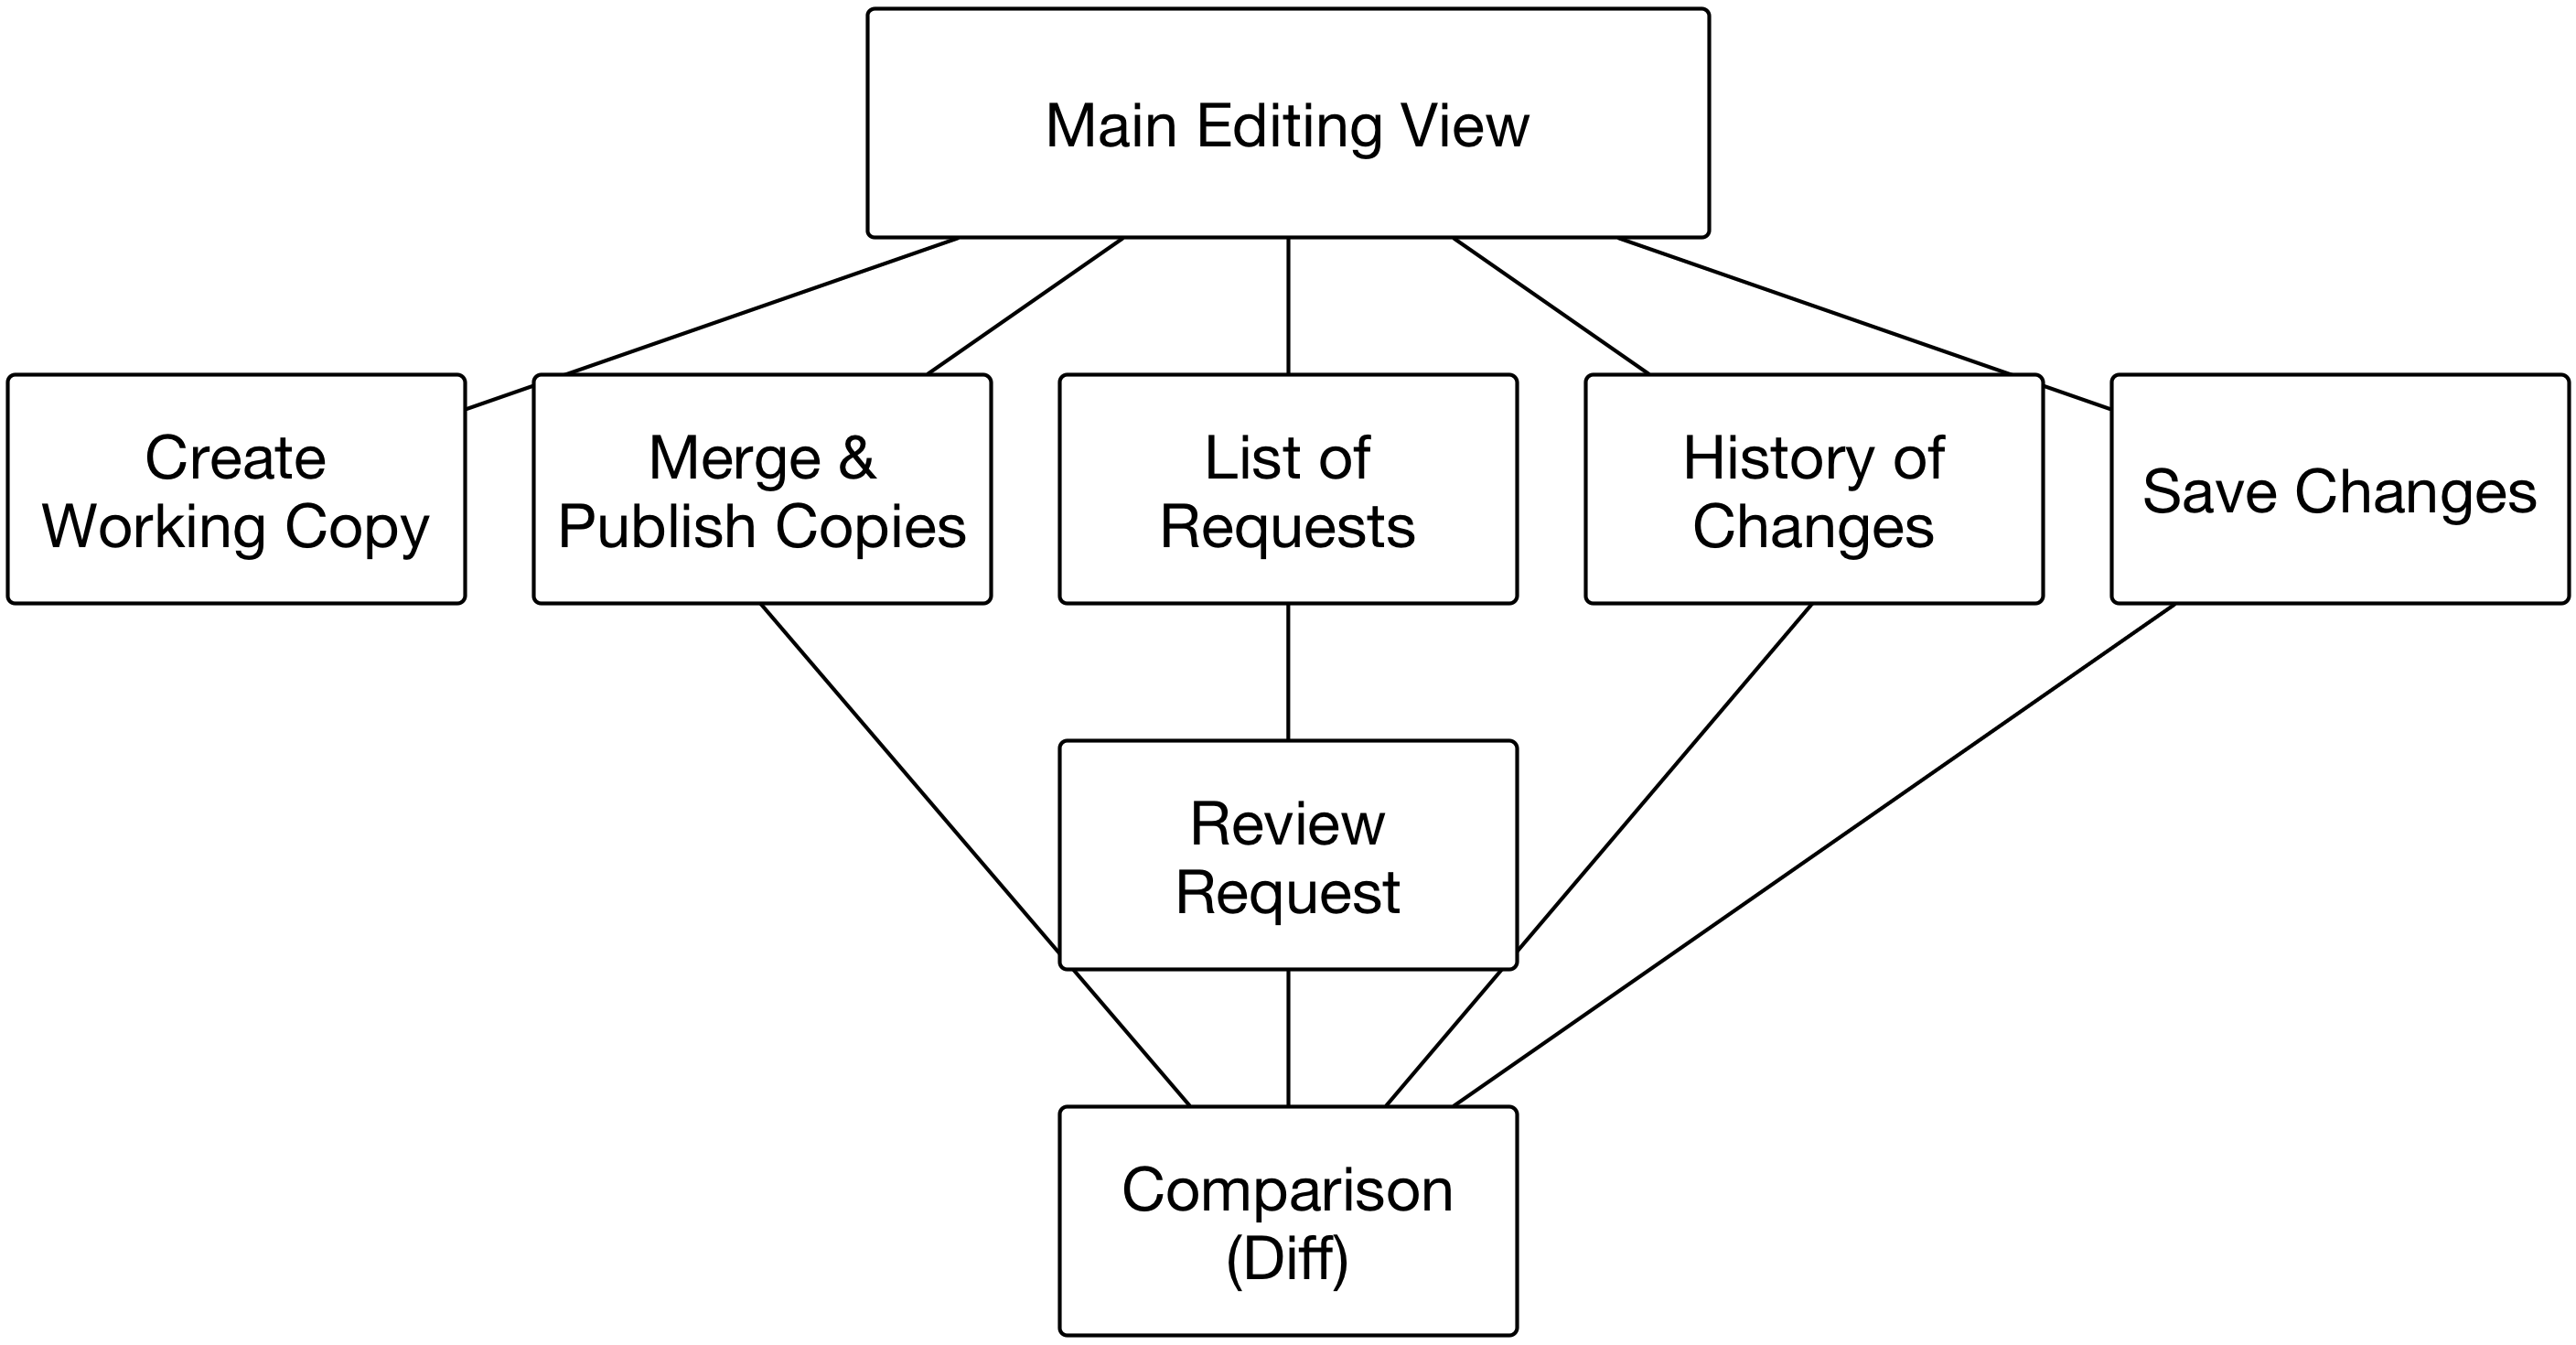
\includegraphics[width=10cm]{second-iteration/main-views-diagram}
 \caption{Overview of main sections of the application}
 \label{fig:main-views-diagram}
\end{figure}

\section{Comparison to Traditional VCSs} \label{sec:git-feature-comparison}
As compared to most other version control systems the interface only offers a minimal set of features. Some of them have been vastly simplified or adapted to the domain of language content authoring. A few features, such as the pull request and the history, are very close to their "originals".

\begin{itemize}
  \item There is no differentiation between \textit{local} and \textit{remote} repositories anymore. Church et al.'s \cite{church_case_2014} work has shown that hidden dependencies between these two repositories often complicate matters for the user. Therefore, it was decided to have only one repository that is constantly up to date. This should, in theory, also simplify collaboration and avoid conflicts.
  \item Specifically \emph{tracking} files is not necessary. Every course or lesson that is created using the tool will be under version control.
  \item There is no \emph{staging} area anymore. As mentioned in Chapter \ref{chapter:related-work} this feature is sometimes problematic and often inconvenient, because every change has to be staged before it can be saved (committed).
  \item The \emph{diff(erence)} view is presented by default before the user saves his or her changes. This ensures that the user knows what will be saved and provides an additional review mechanism. When using the Git CLI, diff is a separate command that needs to be executed when the user wants to look at the things that have changed.
  \item The diff view is enriched by a domain-specific design. It does not only display bare data as represented in the data format, but shows images, allows listening to sounds and visualizes boolean values, so that reviewing changes becomes simpler and is easier for users with a non-technical background.
  \item A \emph{pull request} feature (as on Github) was added. Because Git offers no formalized way of reviewing code before it is merged, this feature enforces best practices. Furthermore, the user analysis has shown that reviewing new content, which was produced by freelancers, is very important.
  %\item Merging is always routed through a pull request, which allows users to review what has changed before merging branches. This reduced the abstraction as compared to merging only based on branch names.
  \item Visualizations were added in order to help users understand some of the more abstract concepts, such as branches. This was inspired by Bitbucket, which is using different visualizations to explain certain features.
\end{itemize}

\section{Prototype}
The overall interface was strongly influenced by existing code hosting platforms, such as Github\footnote{https://github.com/about}, Gitlab\footnote{https://about.gitlab.com/} and Bitbucket\footnote{https://bitbucket.org/} as well as several Git GUIs\footnote{http://git-scm.com/downloads/guis}. The system can be regarded as a crossbreed between version control and content authoring tool. Below, the main views of the prototype are shown.

\subsection{Navigation}
The upper-most navigation bar (Figure \ref{fig:navigation-top}) offers a quick access to the most important version control features as well as the language package and the current branch. Next to the branches dropdown a little plus-icon signifies how a new branch can be created. Furthermore, some buttons provide additional information, such as indicating whether changes can be saved or open pull requests exist.

\begin{figure}[h!]
 \centering
 \fbox{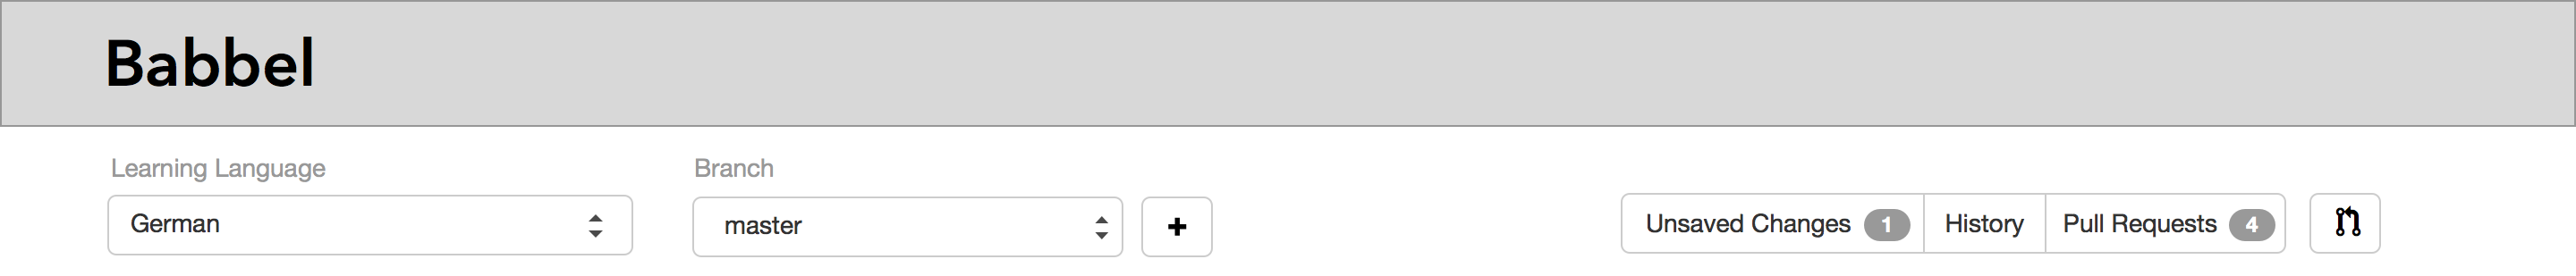
\includegraphics[width=\textwidth]{first-prototype/navigation-top}}
 \caption{The top-bar navigation exposing version control features}
 \label{fig:navigation-top}
\end{figure}

\subsection{Branches}
Branching is a fundamental concept of most version control systems and allows working in an isolated state. A lot of time went into the consideration of whether to include this feature or not. Finally, it was decided, to make this feature visible to users, which has the advantage of them being able to share branches with colleagues or point to a particular state of content that is still being created.

\begin{figure}[h!]
 \centering
 \fbox{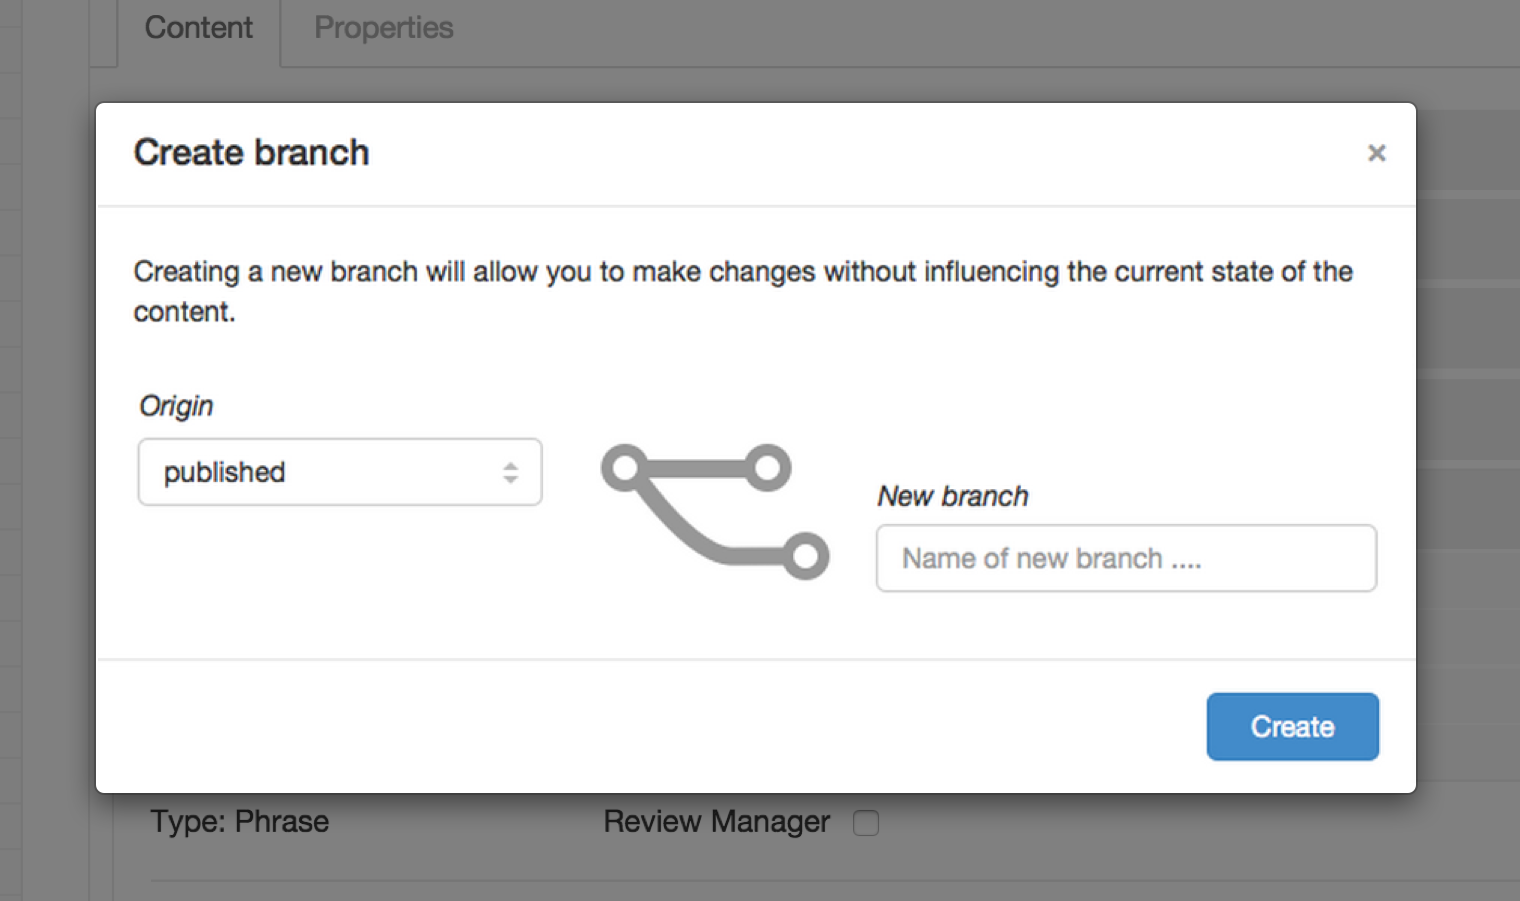
\includegraphics[width=10cm]{first-prototype/create-branch-modal}}
 \caption{The modal allowing users to create new branches}
 \label{fig:create-branch}
\end{figure}

\subsection{Saving Process and Diff View}
As mentioned before, when a user has edited some content, which shall be saved, a difference view is presented. This allows the user to review her changes before committing to a change. As is common with most version control systems, a commit message needs to be entered before saving. This allows collaborators to comprehend why a particular piece of content was edited.

\begin{figure}[h!]
 \centering
 \fbox{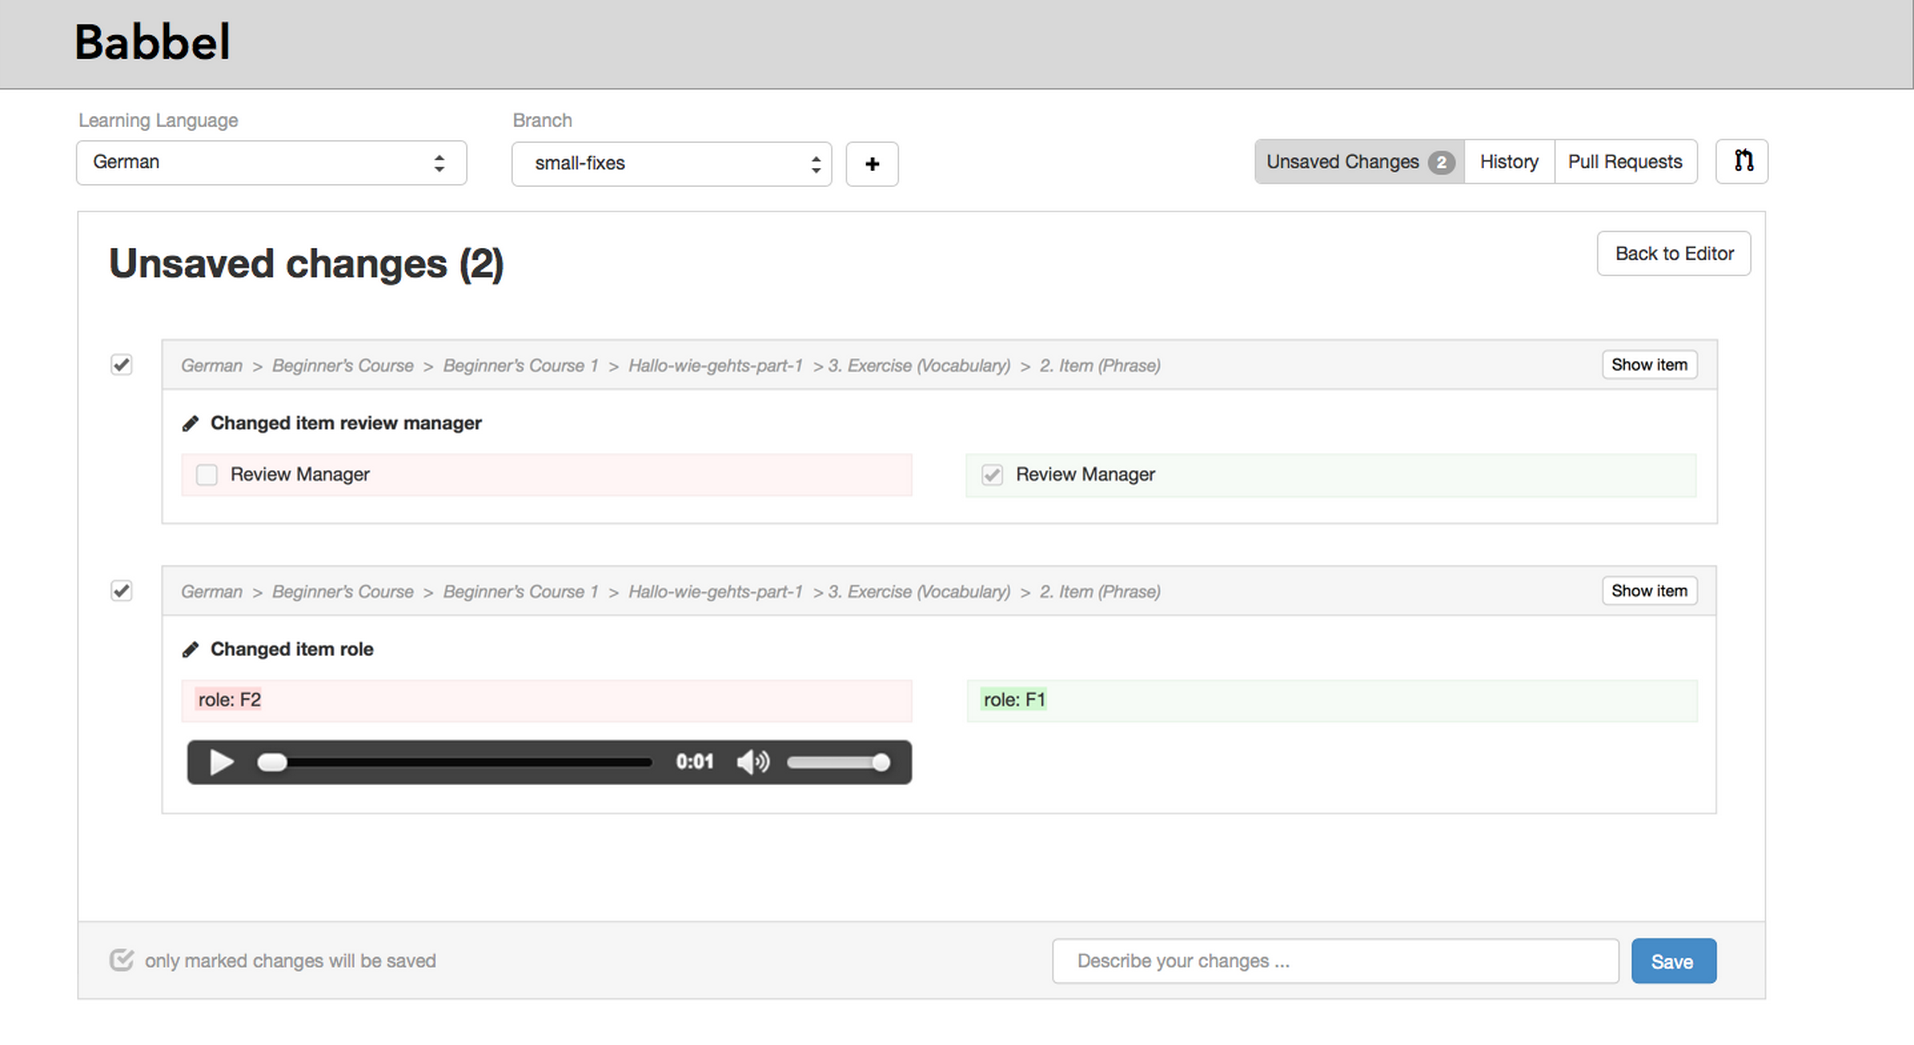
\includegraphics[width=\textwidth]{first-prototype/unsaved-changes}}
 \caption{The difference view highlighting changes the user did recently}
 \label{fig:unsaved-changes}
\end{figure}

\subsection{Content Editing}
The content in the editing view can be navigated by expanding a tree structure (Figure \ref{fig:prot-initial-editor-view}, left-hand side), which also reflects the inherent composition of the content. Furthermore, when a lesson is selected, its exercises are listed and the content can be exposed through so-called accordions. Each exercise consists of several items which themselves consist of text, images and sounds.

\begin{figure}[h!]
 \centering
 \fbox{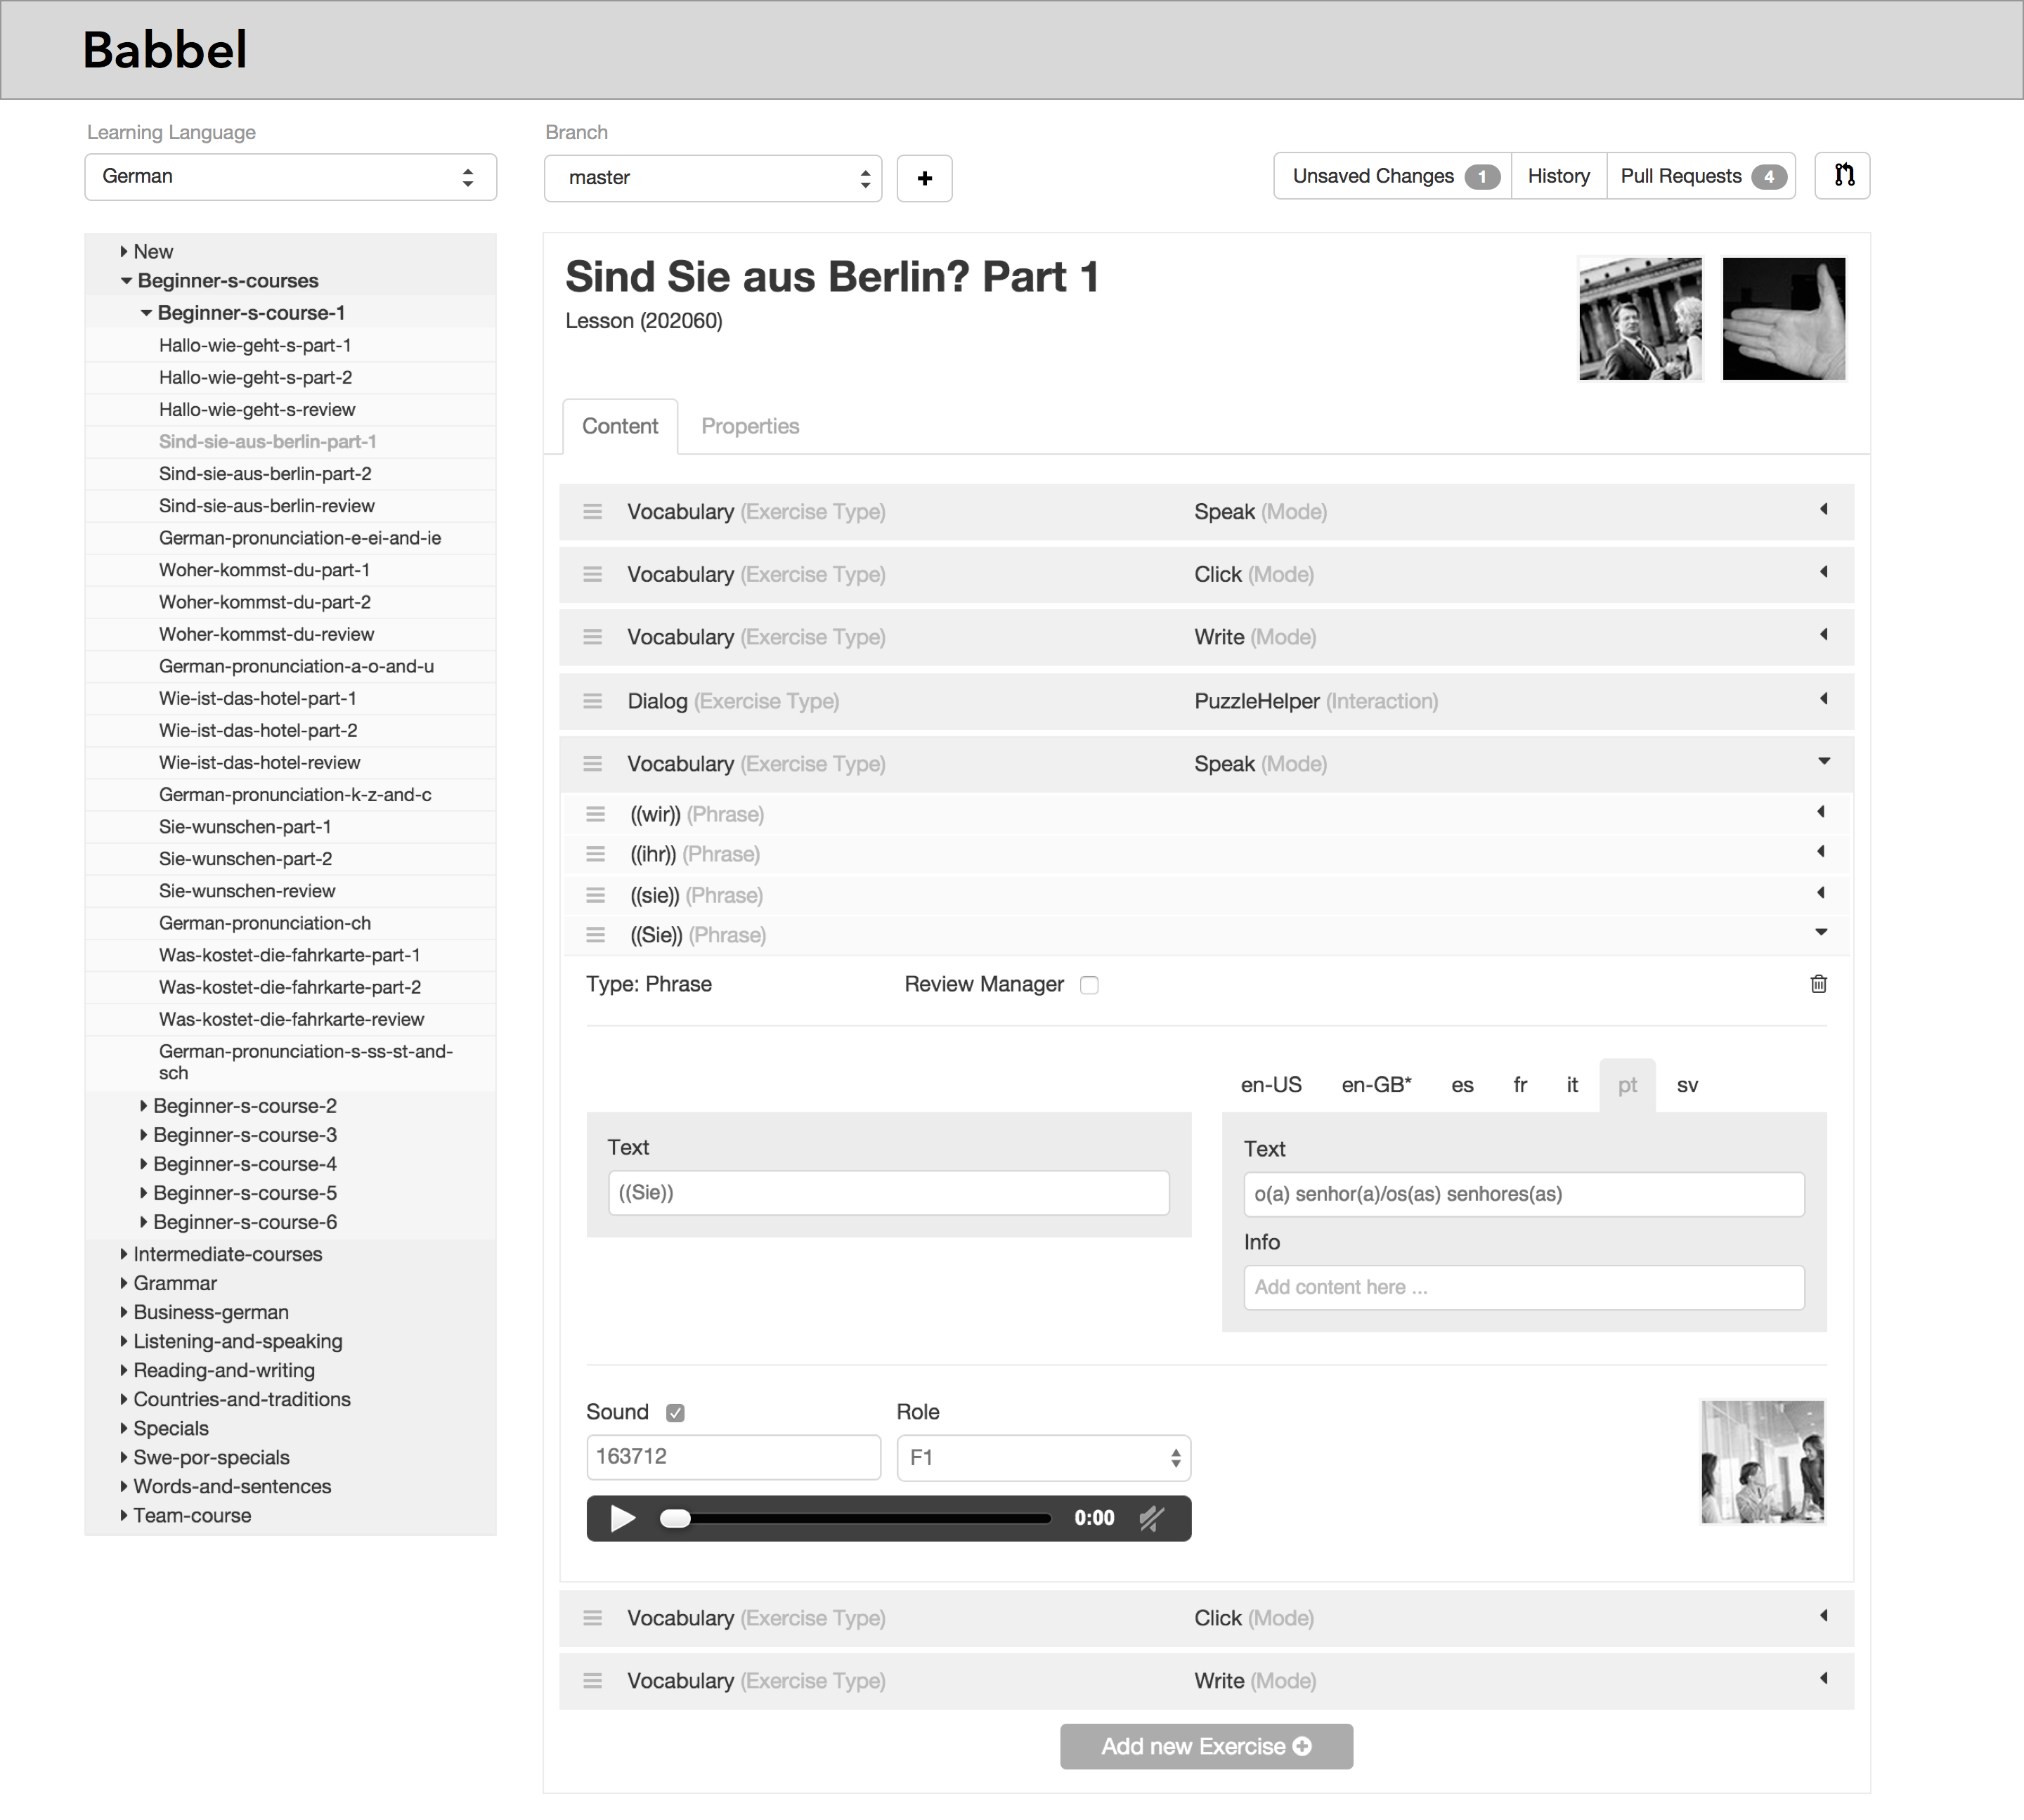
\includegraphics[width=\textwidth]{first-prototype/main-editing-view}}
 \caption{The main editing view with an opened lesson}
 \label{fig:prot-initial-editor-view}
\end{figure}

\subsection{Pull Request}
Pull requests are a formalized way of requesting a "merge" of two branches. A typical version control flow consists of creating a new branch, editing some content, saving it and finally creating a pull request (Figure \ref{fig:open-new-pr}). A pull request allows collaborators to review changes before merging them with the main branch and thus ensures the quality of the content.

\begin{figure}[h!]
 \centering
 \fbox{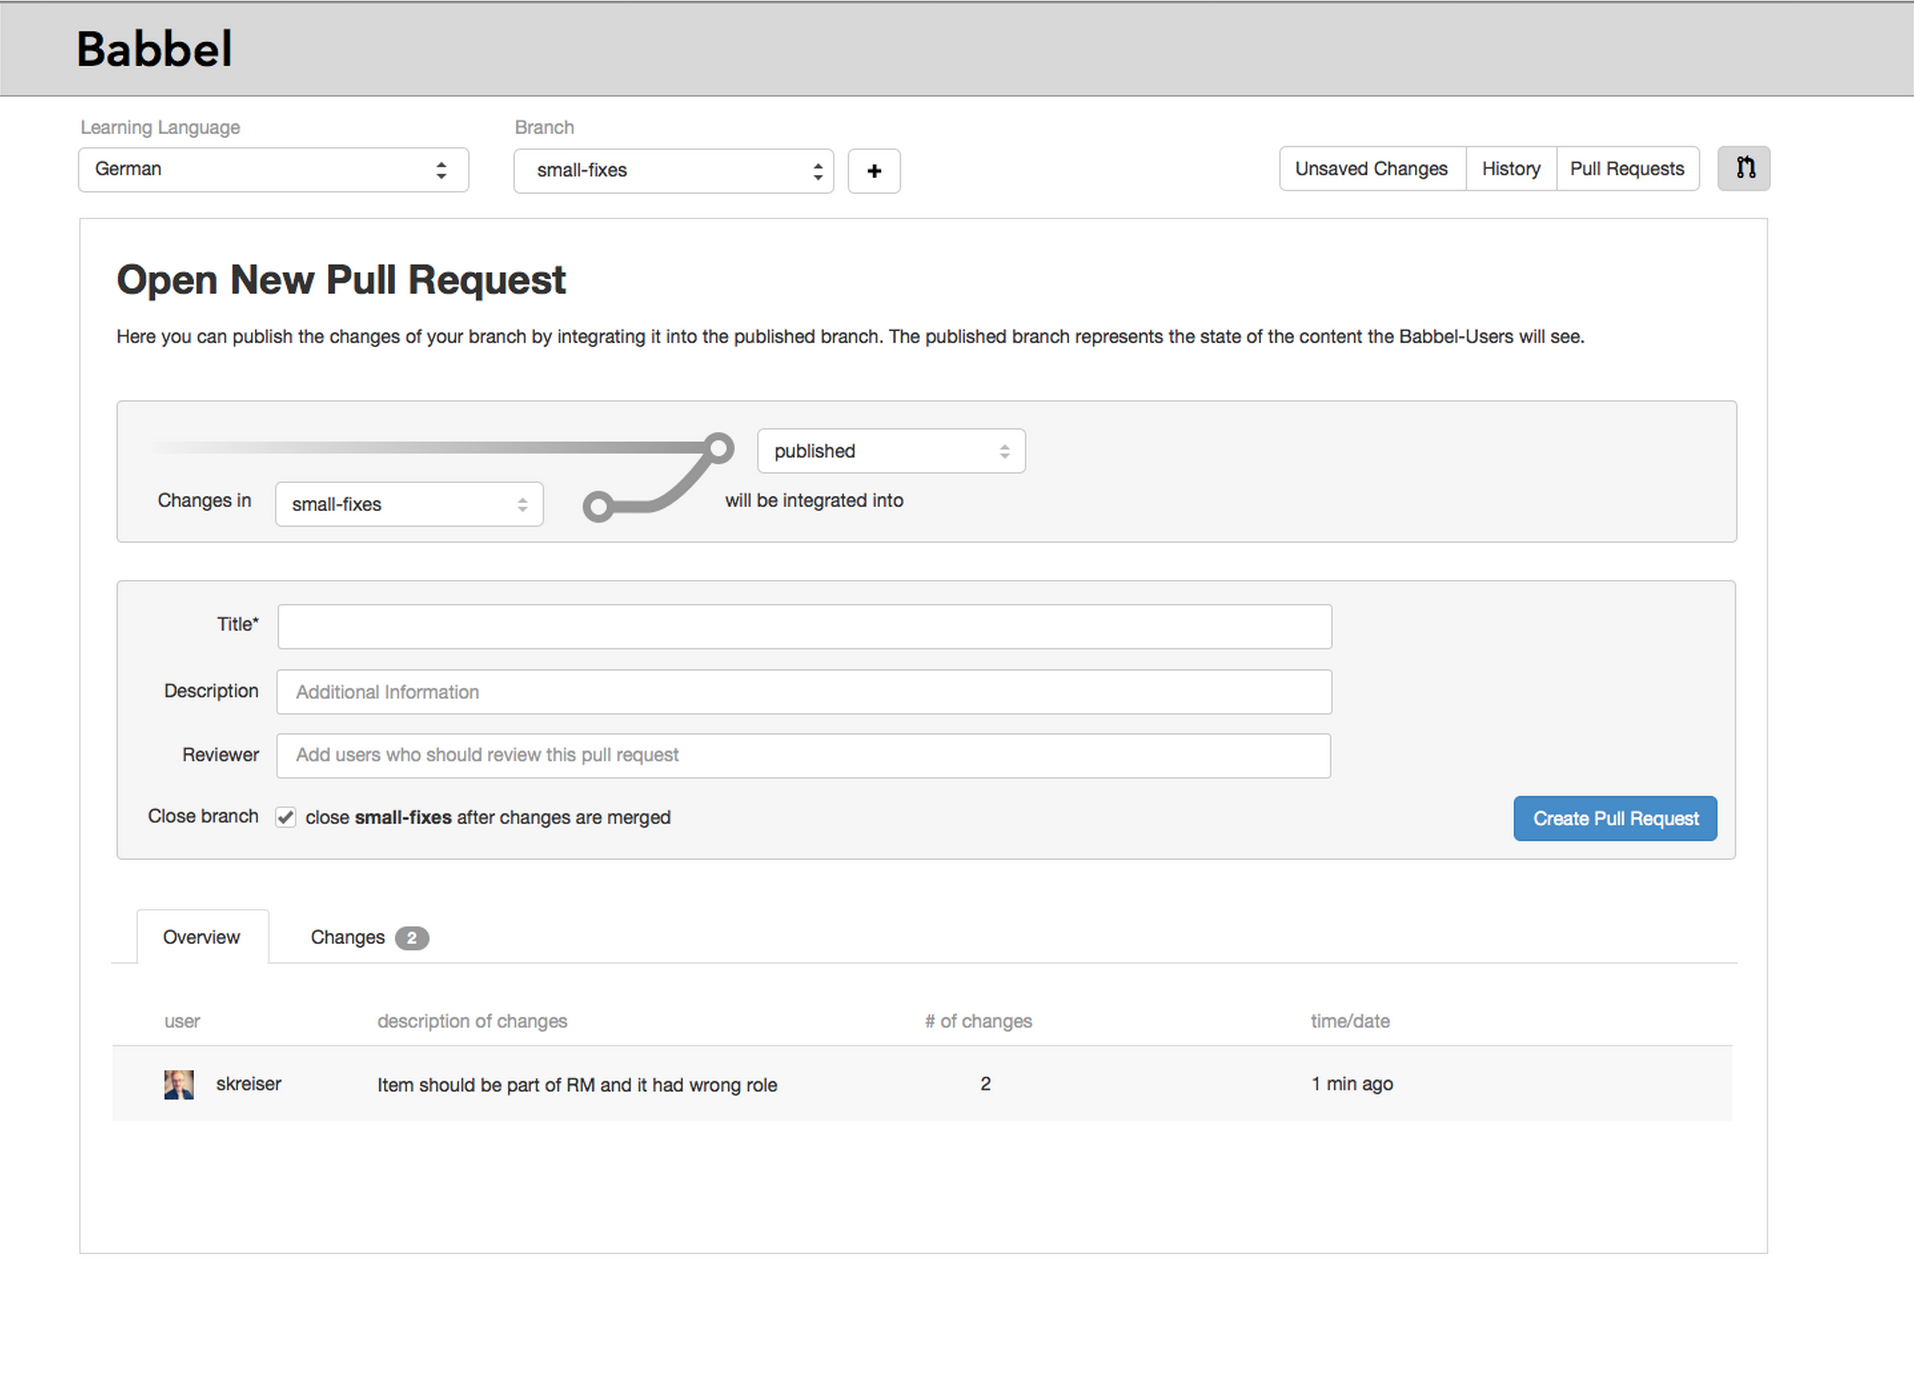
\includegraphics[width=\textwidth]{first-prototype/open-new-pr}}
 \caption{Form allowing the creation of new pull requests}
 \label{fig:open-new-pr}
\end{figure}

% \begin{figure}[h!]
%  \centering
%  \fbox{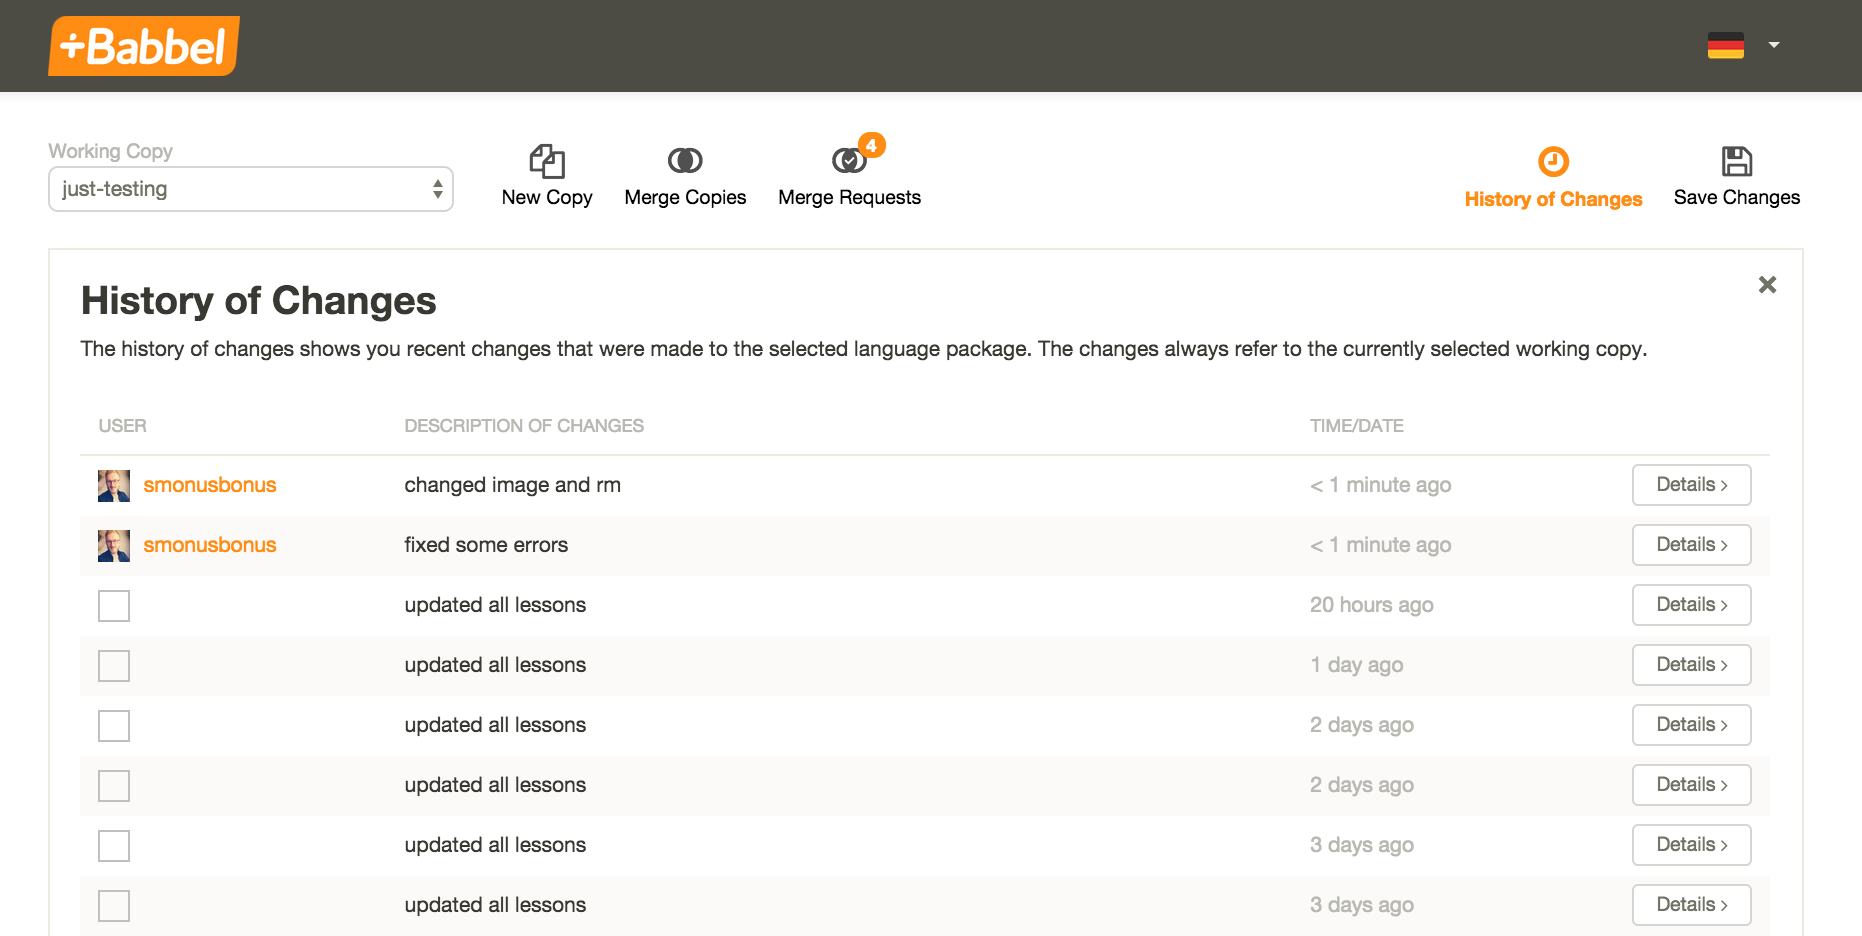
\includegraphics[width=\textwidth]{first-prototype/history}}
%  \caption{The history is a list of recent changes in a particular language package}
%  \label{fig:history}
% \end{figure}


% \begin{figure}[h!]
%  \centering
%  \fbox{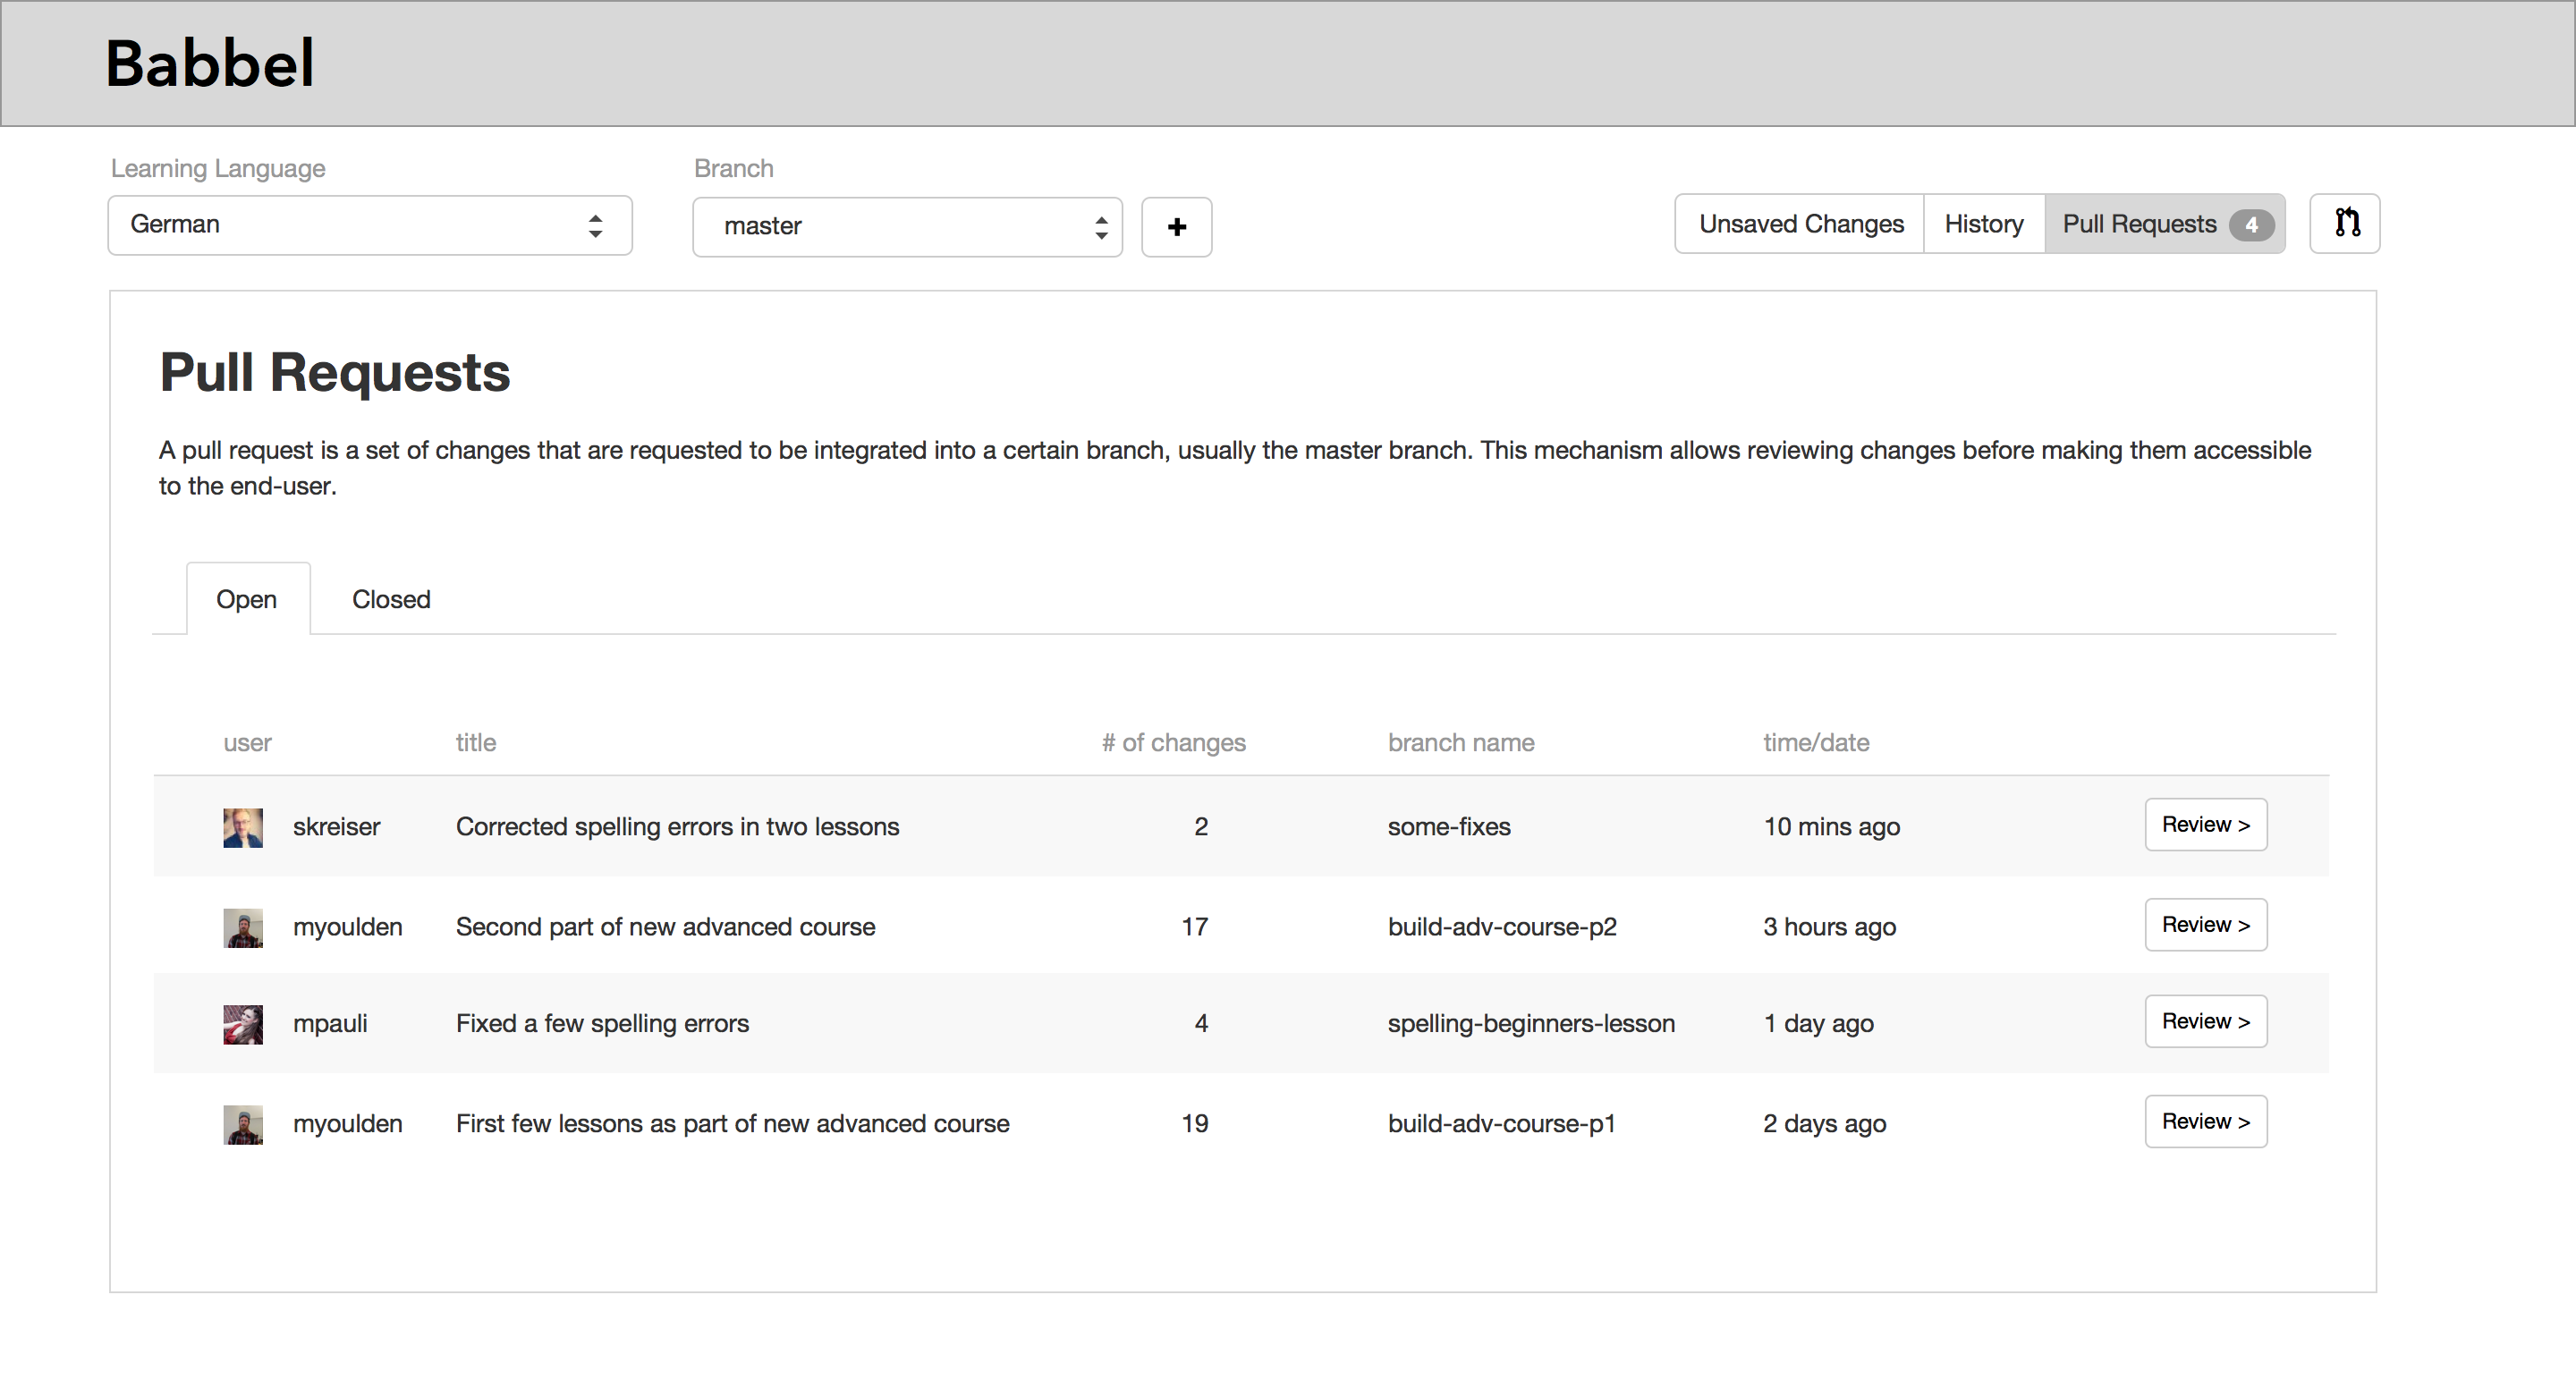
\includegraphics[width=\textwidth]{first-prototype/list-of-pull-requests}}
%  \caption{An overview of existing pull requests}
%  \label{fig:list-of-prs}
% \end{figure}
